% ---------------------------------------------
% Alle Abbildungen 'images/' in Latex speichern 
%     * 'archiv/Pics-files.tex' 
%     * Bildgröße: 0.80/1 
% ju 20-Mär-2021 Pics-files.tex
% ---------------------------------------------
%
%\section{*}
%
%* (\autoref{fig:*}).% Referenz
%
\begin{figure}[!hb]% hier: !hb
    \centering
  \includegraphics[width=.80\textwidth]{images/*.eps}%
  \caption{*}%\label{fig:*}%% anpassen
\end{figure}

%\newpage
%\section{Chili-1}
%
%Chili-1 (\autoref{fig:Chili-1}).% Referenz
%
\begin{figure}[!hb]% hier: !hb
    \centering
  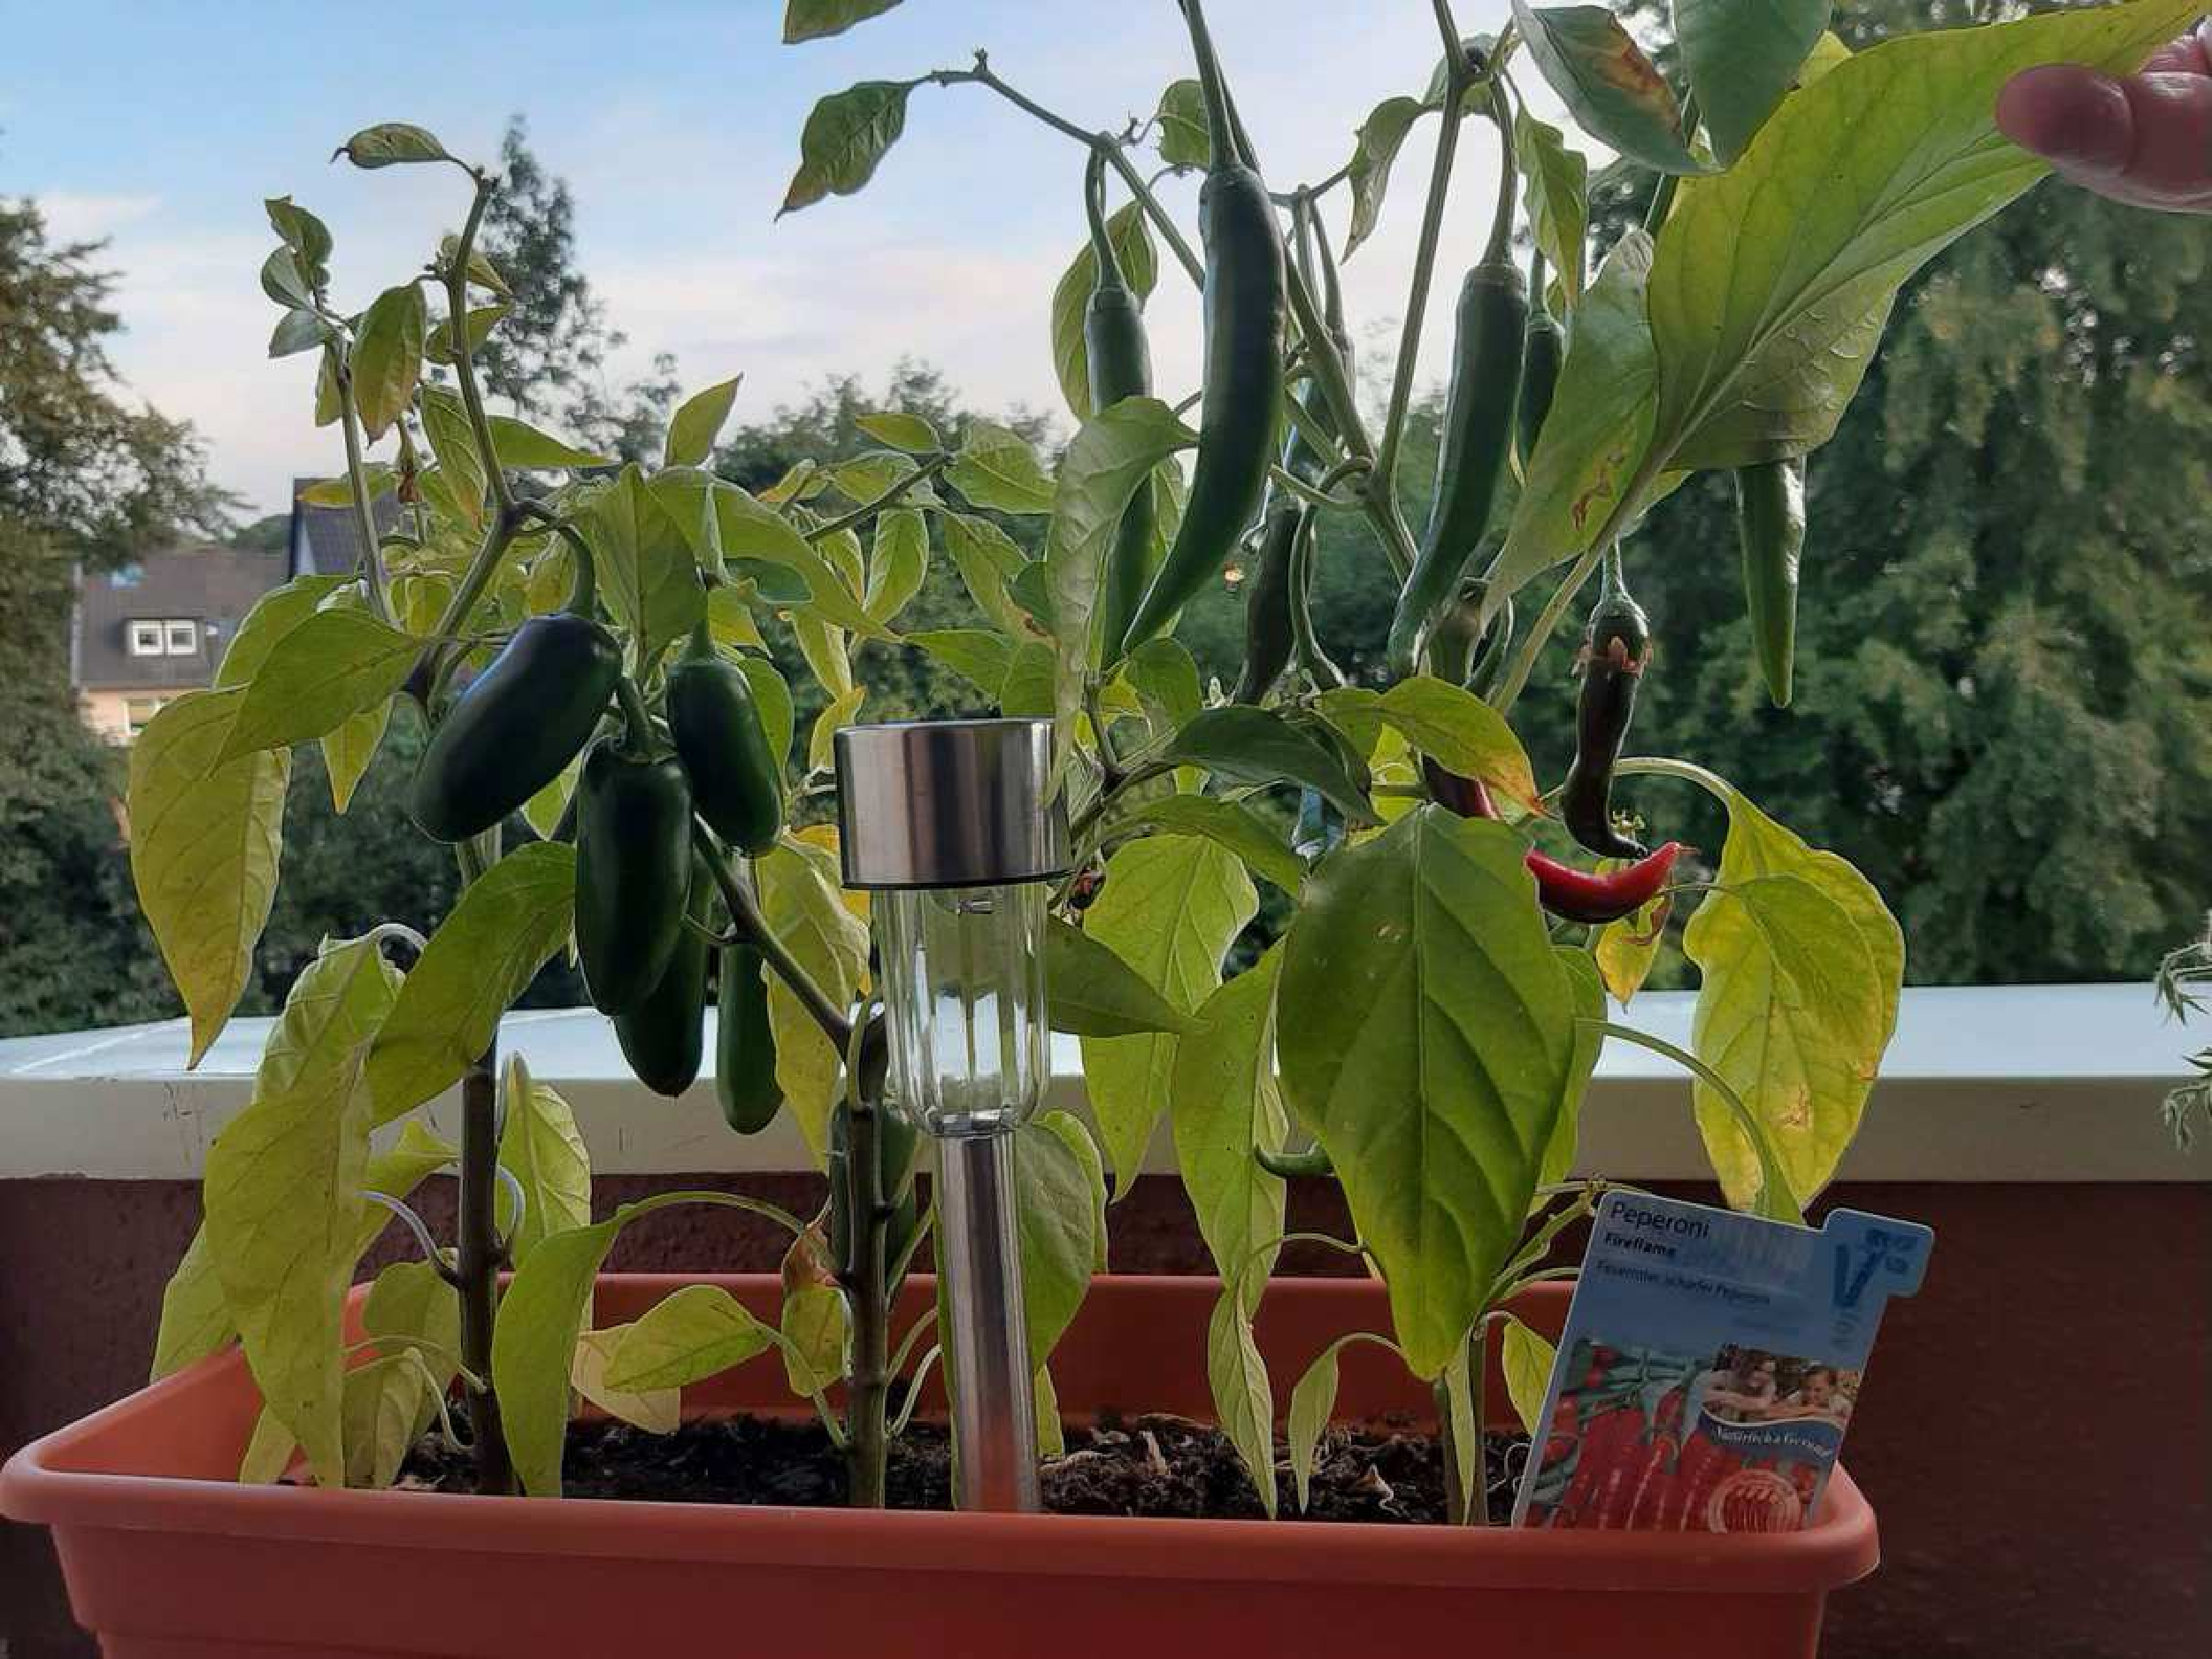
\includegraphics[width=.80\textwidth]{images/Chili-1.pdf}%
  \caption{Chili-1}%\label{fig:Chili-1}%% anpassen
\end{figure}

%\newpage
%\section{logo}
%
%logo (\autoref{fig:logo}).% Referenz
%
\begin{figure}[!hb]% hier: !hb
    \centering
  
\includegraphics[width=.80\textwidth]{Grafiken/logo.eps}%
  \caption{logo}%\label{fig:logo}%% anpassen
\end{figure}

%\newpage
%\section{logo-eps-converted-to}
%
%logo-eps-converted-to (\autoref{fig:logo-eps-converted-to}).% Referenz
%
\begin{figure}[!hb]% hier: !hb
    \centering
  
\includegraphics[width=.80\textwidth]{Grafiken/logo-eps-converted-to.pdf}%
  \caption{logo-eps-converted-to}%\label{fig:logo-eps-converted-to}%% anpassen
\end{figure}

%\newpage
%\section{logo}
%
%logo (\autoref{fig:logo}).% Referenz
%
\begin{figure}[!hb]% hier: !hb
    \centering
  
\includegraphics[width=.80\textwidth]{Grafiken/logo.pdf}%
  \caption{logo}%\label{fig:logo}%% anpassen
\end{figure}

%\newpage
%\section{titelbild-beamer}
%
%titelbild-beamer (\autoref{fig:titelbild-beamer}).% Referenz
%
\begin{figure}[!hb]% hier: !hb
    \centering
  
\includegraphics[width=.80\textwidth]{Grafiken/titelbild-beamer.pdf}%
  \caption{titelbild-beamer}%\label{fig:titelbild-beamer}%% anpassen
\end{figure}

%\newpage
%\section{titelbild}
%
%titelbild (\autoref{fig:titelbild}).% Referenz
%
\begin{figure}[!hb]% hier: !hb
    \centering
  
\includegraphics[width=.80\textwidth]{Grafiken/titelbild.pdf}%
  \caption{titelbild}%\label{fig:titelbild}%% anpassen
\end{figure}

%\newpage
